%%
%% Automatically generated file from DocOnce source
%% (https://github.com/hplgit/doconce/)
%%
%%


%-------------------- begin preamble ----------------------

\documentclass[%
oneside,                 % oneside: electronic viewing, twoside: printing
final,                   % draft: marks overfull hboxes, figures with paths
10pt]{article}

\listfiles               %  print all files needed to compile this document


\usepackage[totoc]{idxlayout}   % for index in the toc
\usepackage[nottoc]{tocbibind}  % for references/bibliography in the toc

\usepackage{relsize,makeidx,color,setspace,amsmath,amsfonts,amssymb}
\usepackage[table]{xcolor}
\usepackage{bm,ltablex,microtype}
\usepackage{comment} 
\usepackage[pdftex]{graphicx}

\usepackage{fancyvrb} % packages needed for verbatim environments

\usepackage[T1]{fontenc}
%\usepackage[latin1]{inputenc}
\usepackage{ucs}
\usepackage[utf8x]{inputenc}

\usepackage{lmodern}         % Latin Modern fonts derived from Computer Modern


\usepackage{pgfplotstable, booktabs}

\pgfplotstableset{
    every head row/.style={before row=\toprule,after row=\midrule},
    every last row/.style={after row=\bottomrule}
}





% Hyperlinks in PDF:
\definecolor{linkcolor}{rgb}{0,0,0.4}
\usepackage{hyperref}
\hypersetup{
    breaklinks=true,
    colorlinks=true,
    linkcolor=linkcolor,
    urlcolor=linkcolor,
    citecolor=black,
    filecolor=black,
    %filecolor=blue,
    pdfmenubar=true,
    pdftoolbar=true,
    bookmarksdepth=3   % Uncomment (and tweak) for PDF bookmarks with more levels than the TOC
    }
%\hyperbaseurl{}   % hyperlinks are relative to this root

\setcounter{tocdepth}{2}  % levels in table of contents

% --- fancyhdr package for fancy headers ---
\usepackage{fancyhdr}
\fancyhf{} % sets both header and footer to nothing
\renewcommand{\headrulewidth}{0pt}
\fancyfoot[LE,RO]{\thepage}
% Ensure copyright on titlepage (article style) and chapter pages (book style)
\fancypagestyle{plain}{
  \fancyhf{}
  \fancyfoot[C]{{\footnotesize \copyright\ 1999-2018, "Computational Physics I FYS3150/FYS4150":"http://www.uio.no/studier/emner/matnat/fys/FYS3150/index-eng.html". Released under CC Attribution-NonCommercial 4.0 license}}
%  \renewcommand{\footrulewidth}{0mm}
  \renewcommand{\headrulewidth}{0mm}
}
% Ensure copyright on titlepages with \thispagestyle{empty}
\fancypagestyle{empty}{
  \fancyhf{}
  \fancyfoot[C]{{ }}
  \renewcommand{\footrulewidth}{0mm}
  \renewcommand{\headrulewidth}{0mm}
}

\pagestyle{fancy}


% prevent orhpans and widows
\clubpenalty = 10000
\widowpenalty = 10000

% --- end of standard preamble for documents ---


% insert custom LaTeX commands...

\raggedbottom
\makeindex
\usepackage[totoc]{idxlayout}   % for index in the toc
\usepackage[nottoc]{tocbibind}  % for references/bibliography in the toc
\usepackage{listings}
\usepackage[normalem]{ulem} 	%for tables
\useunder{\uline}{\ul}{}
\usepackage{hyperref}
\usepackage[section]{placeins} %force figs in section

%-------------------- end preamble ----------------------

\begin{document}

% matching end for #ifdef PREAMBLE

\newcommand{\exercisesection}[1]{\subsection*{#1}}


% ------------------- main content ----------------------



% ----------------- title -------------------------

\thispagestyle{empty}

\begin{center}
{\LARGE\bf
\begin{spacing}{1.25}
Simulating the The Ising model using the Metropolis algorithm
\end{spacing}
}
\end{center}

% ----------------- author(s) -------------------------

\begin{center}
{\bf Johan Nereng}
\end{center}

    \begin{center}
% List of all institutions:
\centerline{{\small Department of Physics, University of Oslo, Norway}}
\end{center}
    
% ----------------- end author(s) -------------------------

% --- begin date ---
\begin{center}
Sep 24, 2018
\end{center}
% --- end date ---

\vspace{1cm}
The Stern Gerlach experiment in \newline
\section{Abstract}

\section{Introduction}
In general, magnets are objects which produce a magnetic field. Such fields arise from net magnetic moment and induction from electric currents  \cite{FeynmanMM}. In the case of the strong magnetic fields observed in ferromagnets, the spin configuration of electrons in neighboring atoms largely decides the net magnetic moment \cite{FeynmanFM}. This means that there is a connection between the microstate of the object and it's magnetic properties. These microstates are quantum states, and are therefore of a stochastic nature. The probability of a system occupying a specific microstate, may therefore be described in the canonical ensemble by the Boltzmann distribution \eqref{eq:Boltzdist} where $k_B$ is the Boltzmann constant, $T$ the temperature,  and $Z$ \eqref{eq:partitionfunction} the canonical partition function, which sums over the energy, $E$, of all possible states \cite{HJ-SP}. 

\begin{equation}
P_i(\beta)=\frac{e^{-\beta E_i}}{Z}, \text{ where }\beta=1/k_BT 
\label{eq:Boltzdist}
\end{equation}

\begin{equation}
Z=\sum_{i=1}^M e^{-\beta E_i}
\label{eq:partitionfunction}
\end{equation}

The properties of the canonical ensemble is used to find the expectation value of the energy, $\langle E \rangle$ which is subject to both the principle of energy minimization and the principle of maximum entropy, $S$. At the equilibrium point between these principles, the Helmoltz' free energy, $F=\langle E \rangle-TS$, is minimized [ibid]. In addition, a ferromagnetic object loses it's magnetic properties at a certain critical temperature known as the Curie Temperature, $T_C$, which may also be used to describe phase transition between ferromagnetism and paramagnetism \cite{FeynmanFM}. Thus, in order to examine such phase transitions in ferromagnets, this project empathizes mean energy, temperature, and net magnetization, as well as two additional parameters; specific heat capacity at constant volume, $C_V$, which are related to the derivative of the Helmholt'z free energy \cite{HJ-SP}, and the magnetic susceptibility, $\chi$, which quantifies the material's response to an external magnetic field. \newline

The projects start by describing the \hyperref[SS:thermodynamic.properties]{thermodynamic properties} of the magnetic system are described, and expressions for $\langle E \rangle$, $C_V$, $\langle M \rangle$, and $\chi$. Next, the mathematical model known as the \hyperref[SS:Ising]{the Ising model}, utilizing a two dimensional lattice of size $L \times L$ is introduced and briefly explained. Then, this model is \hyperref[SS:M.Model_application]{applied to a magnetic system} of atom spins, and analytical expressions as functions of the temperature, $T$, are derived for an $L=2$ lattice, using the mean absolute value of the magnetic moment  $\langle |M| \rangle$ in addition to the previously mentioned properties.  \newline

Having outlined the mathematical basis for the project, a Markov Chain Monte Carlo method known as the \hyperref[SS:MCMCmethod]{Metropolis algorithm} is  applied to the system in order to simulate the magnetic properties described by the Ising model. This algorithm is subsequently \hyperref[SS:init.algo.impl]{implemented} in a \textit{C++} program, and the simulation results for an $L=2$ lattice \hyperref[SS:R.initialeval]{compared} with the analytical values for $T=1$, which indicated that sufficiently accurate expectation values were produced after an equilibrium time $t_{eq} \approx 3 \cdot 10^6$ Monte Carlo cycles. \newline

Upon having established algorithm integrity through the initial test described above,\hyperref[SS:M.Eq.time]{$t_{eq}$ is further examined}, and the effects of initial spin configuration (random or ordered) looked into. 


\hyperref[SS:M.variance ]{the Ising model}
\hyperref[SS:M.Phase_trans]{the Ising model}
\hyperref[SS:Est.Curie]{the Ising model}

SS:results.VAR 
SS.R.EQtime 
SS:R.initialeval
SS.estCurie
$k_B T$ - is temp!


2.3 not 2.4 as 2.3 is used in the last, and not 2.4. 
\section{Methods}

\begin{comment}
- Brief description of magnets (finn en kilde)
	- magnetic properties in relation to spin- stern gerlach -> sammenheng mellom spinn og magnetisme (ikke grei ut mye)
	- Sammenheng mellom temp og magnetisk egenskaper (M) -> faseovergang
	- Energy relatert til SS av systemet - stabilty->ss. Helmholtz free. Ser på magnet om isolert system -> må ha med varmekap.
	-critical temp on magnets - lose magn. properties in phase 	 		transition ( exact critical temp Lars Onsager)
	- mål på faseovergang: varmekap, mag. susc, chi (reponse of magnet to ext. mag field) 
\end{comment}

\subsection{Thermodynamic properties}
\label{SS:thermodynamic.properties}	
As the ferromagnetic system in this project is described through the 
canonical ensemble, the energy \eqref{eq:Eexp} and magnetization \eqref{eq:Magnetization} of the ferromagnet are expectation values, the expressions of which are derived via the Helmoltz' free energy and entropy in the canonical ensemble \cite{HJ-SP}. 


\begin{equation}
\langle E \rangle = \sum_i^M E_i P_i (\beta)
\label{eq:Eexp}
\end{equation}

\begin{equation}
\langle M \rangle=\sum_i^M M_i P_i (\beta)
\label{eq:Magnetization}
\end{equation}

Through the expectation values above, the specific heat capacity at constant volume, $C_V$ \eqref{eq:specificheat}, signifying the amount of heat needed to change the temperature of the system, and the magnetic susceptibility, $\chi$ \eqref{eq:Magsuscept}, which quantifies the response to an external magnetic field, are defined. 

\begin{equation}
C_V=\frac{1}{k_B T^2} (\langle E^2 \rangle - \langle E \rangle^2 )
\label{eq:specificheat}
\end{equation}

\begin{equation}
\chi=\frac{1}{k_B T}(\langle M^2 \rangle - \langle M \rangle^2 )
\label{eq:Magsuscept}
\end{equation}	

\subsection{The Ising model}   
\label{SS:Ising}	
In order to simulate ferromagnetic behaviour and properties, this project employs a theoretical description of ferromagnets known as the Ising model. This model consists of $L \times L$ binary variables on a two dimentional lattice, representing identical spin systems, with the energy of a specific spin configuration, or microstate, $i$ defined as \cite{Fitzpatrick}:
\begin{equation}
E_i=-J\sum_{\langle kl \rangle} s_k s_l -B \sum_{i=k} s_k
\end{equation} 
Where, $J>0$ is the exchange energy, $B$ external magnetic field, and $s_k$, $s_l$, the $k$'th and $l$'th atomic spins of a total of $N$ spins. The sum over ${\langle kl \rangle}$ is the sum over unique neighbouring spin pairs, while the spins are either spin up ($\uparrow $), $s=+1$, or spin down ($\downarrow $), $s=-1$ [ibid].  As this project aims to study phase transition in a ferromagnet without any external magnetic field, $B=0$, so that:
\begin{equation}
E_i=-J\sum_{\langle kl \rangle} s_k s_l 
\label{eq:IsingEnergy}
\end{equation} 

In addition to the energy, the Ising model is defined through the magnetization of configuration $i$, defined as:
\begin{equation}
M_i=\sum_{k} s_k  
\end{equation}

In order to define the end points of the lattice, this project utilizes of periodic boundary conditions, which means that $s_{n(L+1)}=s_{n}$, where $n=1,2..,L$, which is to say that the lattice may be viewed as the surface of a torus.  

\subsection{Model application - benchmarking}
\label{SS:M.Model_application}
With the aim of obtaining evaluation parameters for the implementation of the later described Marcov Chain Monte Carlo method (\hyperref[SS:MCMCmethod]{the Metropolis algorithm}), the analytical expressions for $\langle E \rangle$, the expectation value of the absolute magnetic moment $|M|$ \eqref{eq:meanabsM}, $C_V$, and $\chi$, as functions of the temperature, $T$, are derived for a $2 \times 2$ lattice. This requires working out the  partition function, $Z$, which depends on the number of spin configurations and their corresponding energy values. In addition, deriving the expression for $\chi$ hinges on knowing the magnetization of each spin configuration. \newline

\begin{equation}
\langle M_i \rangle =\sum_{k} |s_k| P_i(\beta)
\label{eq:meanabsM}
\end{equation}

The spin configurations for the $2 \times 2$ Ising model lattice, and their energies and magnetization, are presented in table \ref{tab:states}, where the degeneracy number signifies the number of spin configurations with the same energy and magnetization levels. Based on this table and equations \eqref{eq:Eexp}, \eqref{eq:meanabsM}, \ref{eq:specificheat}, \eqref{eq:partitionfunction} the analytical expressions for the $2 \times 2$ lattice are presented below. Using these, the evaluation parameters (per spin) for $T=1$ are presented in table \ref{tab:analytical_values}, under \hyperref[SS:init.algo.impl]{Algorithm implementation}.\newline

\begin{table}[h!tb]
    \centering
    \caption{Overview of microstates for a $2x2$ lattice}
\pgfplotstableset{% global config, for example in the preamble
% these columns/<colname>/.style={<options>} things define a style
% which applies to <colname> only.
empty cells with={--}, % replace empty cells with ’--’
every head row/.style={before row=\toprule,after row=\midrule},
every last row/.style={after row=\bottomrule}
}
\pgfplotstabletypeset[ % local config, applies only for this table
1000 sep={\,},
columns/info/.style={
fixed,fixed zerofill,precision=1,showpos,
column type=r,
}
]
{states.dat}
\label{tab:states}
\end{table}

\begin{align}
Z(T)&=12+2(e^{\frac{-8J}{k_B T}}+e^{\frac{8J}{k_B T}})=12+4 cosh(\frac{8J}{k_B T}) \label{eq:Z(T)}\\
\langle E \rangle (T)&= \frac{16}{Z}( e^{\frac{-8J}{k_B T}} -e^{\frac{8J}{k_B T}})J \\
\langle |M| \rangle (T)&=\frac{8}{Z}(e^{\frac{8J}{k_B T}}+1) \\
\chi (T)&=\frac{1}{k_BT}(\frac{32}{Z}(e^{\frac{8J}{k_B T}} +1)\\
C_V (T)&=\frac{1}{k_BT} \big( \frac{256}{Z} cosh(\frac{8J}{k_B T}) -\frac{32^2}{Z^2}cosh^2(\frac{8J}{k_B T})\big) \label{eq:C_v(T)}
\end{align} 

\textit{In order to obtain expectation values per spin, the equations above must be divided by $L^2$.}


\subsection{The Metropolis algorithm}
\label{SS:MCMCmethod}
Calculating the partition function of a lattice of any significant size is impractical, bordering on the impossible, so in order to numerically model the ferromagnet, a Markov Chain Monte Carlo (MCMC) method is applied, namely the Metropolis algorithm. This method takes an initial spin configuration, proposes a new spin configuration, and either accepts or rejects the new configuration based on it's sampling rule. By relying solely on the relative likelihood of a proposed configuration relative to the current configuration, the metropolis algorithm circumvents the partition function. Over the course of a large number of proposed configuration changes, the system reaches an equilibrium state - in which the spin configuration, energy and magnetization fluctuates around a mean as a function of temperature, enabling the study of the ferromagnetic properties without ever using the partition function. Below is a brief summery of the algorithm \cite{HJ-SP}, and thereafter an augmenting description it. 


\begin{center}\fbox{\parbox{\textwidth}{{\textbf{MCMC: Metropolis algorithm}}
\begin{enumerate}
\item Initialize lattice
\subitem - Set the spin orientation of starting configuration.
\subitem - Calculate $E$ and $M$
\item Propose new configuration (see comments below about lattice sweep)
\subitem - Generate a random spin index $k$. 
\subitem - Set $s_k=-s_k$.
\subitem - Calculate $\Delta E$
\item Evaluate proposal
\subitem - If $\Delta E \leq 0$, accept the new configuration (update $E$ and $M$) and move to step 4.
\subitem - Generate a random number $r$ between $0$ and $1$. 
\subitem - If $r\leq e^{-\beta \Delta E}$, accept new configuration (update $E$ and $M$).
\subitem - If proposed configuration has not been accepted, reject proposal, and set $s_k=-s_k$ (dial-back configuration).
\item Update $E_{total}$, $M_{total}$, $E^2_{total}$, $M^2_{total}$, $|M|_{total}$
\item If the number of cycles from step $2$ to $4$ is less than the total number of $MCc$, go to step 2. Else calculate $\langle E \rangle, \langle E^2 \rangle, \langle M \rangle,\langle M^2 \rangle, \langle |M| \rangle$ and end simulation.  
\end{enumerate}}}\end{center}

When initializing the lattice in step 1, this project employs both an ordered initial spin configuration (all spins $\uparrow$), and a randomized configuration, in which the orientation of each spin is randomized. Furthermore the metropolis algorithm is applied with the use of lattice sweeps. This means that prior to step 4, $L \times L$ uniformly distributed spin indexes, $k$ are generated. For each such index, the algorithm goes through step 2 and 3 for each such $k$, before moving on to step 4, where the change in each quantity is simply added to the corresponding sum. At step 5, in order to find $E_{total}$, $M_{total}$, $E^2_{total}$, $M^2_{total}$, $|M_{total}$, and based on these, $\chi$ and $C_V$, $E_{total}$, $M_{total}$, $E^2_{total}$, $M^2_{total}$, $|M|_{total}$ are divided by the number of Monte Carlo cycles (lattice sweeps), and the number of spins. This means that all values extracted from the simulation are per spin.  \newline


The energy change, $\Delta E$ in it's easiest form simply takes the difference between current energy from \eqref{eq:IsingEnergy} and proposed energy. However, as the spins are only changed on at the time, there is no need to keep track of the energy of the current state in order to work out $\Delta E$ - it may after all only take on five possible values: $-8J, -4J, 0J,4J, 8J$  \cite{HJ-SP} - which means that the temperature really only affect the sampling rule $r\leq e^{-\beta \Delta E}$. Lastly, it's worth mentioning that this Metropolis algorithm set up ensures ergodicity and detailed balance, which may be read about in more detail in 
"An introduction to Monte Carlo methods" by J.C.Waltera and G.T.Barkema\cite{Walter}.


\subsection{Algorithm implementation}
\label{SS:init.algo.impl}	
The MCMC algorithm is now implemented into program through code written in \textit{C++} with the armadillo library \cite{armadillo}, using the template for the Ising model with the Mersenne twister random number engine from the Github page of the course Computational Physics at the University of Oslo \cite{CPgithub}. \newline

In order to test the integrity of the algorithm in the program implementation, the program is run with $L=2$, initial configuration as all spins up, $T=1$, and $MCc=10^8$. The results for $\langle E \langle$, $\langle |M| \rangle$, $\chi$, and $C_V$ are then plotted as functions of the number Monte Carlo cycles, and compared to the analytical values obtained from \eqref{eq:Z(T)} through \eqref{eq:C_v(T)} presented in table \ref{tab:analytical_values}, with the intention of establishing the magnitude of the number of cycles needed to obtain a tolerable precision. The results are expected to fluctuate and deviate less from the analytical values as the number of Monte Carlo cycles approaches the required number to obtain a stable equilibrium state.\newline



\begin{table}[h!tb]
    \centering
    \caption{Analytical values for $2x2$ lattice for $T=1$}
\pgfplotstableset{% global config, for example in the preamble
% these columns/<colname>/.style={<options>} things define a style
% which applies to <colname> only.
columns/E/.style={fixed zerofill,precision=4,column name=\textsc{$\langle E \rangle  $}},
columns/M/.style={precision=6,column name=\textsc{$\langle |M| \rangle  $}},
columns/X/.style={precision=6,column name=\textsc{$\chi  $}},
columns/C/.style={precision=6,column name=\textsc{$C_V  $}},
empty cells with={--}, % replace empty cells with ’--’
every head row/.style={before row=\toprule,after row=\midrule},
every last row/.style={after row=\bottomrule}
}
\pgfplotstabletypeset[ % local config, applies only for this table
1000 sep={\,},
columns/info/.style={sci zerofill
}
]
{analytical_values.dat}
\label{tab:analytical_values}
\end{table}
 
\subsection{Equilibrium time}
\label{SS:M.Eq.time}
The program is now more closely examined with respect to equilibrium time - the number of cycles needed to reach stable expectation values. After  \hyperref[SS:Disucssion_init_eval]{establishing an initial estimate} of the equilibrium time of $3\cdot 10^6$ cycles, the first step is evaluating the equilibrium time of $C_V$ for a larger lattice ($L=20$, $T=1$), as $C_V$ had one order of magnitude larger relative error than $\chi$ the initial tests. After this, the effects of initial spin configuration on equilibrium time is examined by comparing a random initial orientation versus an ordered orientation (all spins $\uparrow$). This is done by evaluating the time/cycle evolution of $\langle E \rangle$ and $\langle |M| \rangle$ for a $L=20$ lattice over $4 \cdot 10^6$ cycles, examining both $T=1$ and $T=2.3$ - the lowest and highest temperatures used later in this project - with emphasis on convergence to equilibrium means.  \newline

The initially estimated equilibrium time is based on the stability of the expectation values for $L=2$, which means that it should be more than sufficient for larger lattices. A confirmation of this is however needed before moving on to phase transitions. Lastly, the effects of temperature on the number of accepted spin configurations is looked into. As the sampling rule yields increased acceptance rate for increased temperatures, the number of accepted configurations is expected to exponentially increase with $k_b T$. 

 
\subsection{Variance in energy}
\label{SS:M.variance}
Having established an equilibrium time of $3 \cdot 10^6$, the algorithm implementation is now tested with respect to the variance of energy,  $\sigma_E^2$. This is done by setting up a $L=40$ lattice, and counting the number of energies of the system after equilibrium state is achieved. Based on the distribution of energies, $P(E)$ is calculated, and the results compared to the standard deviation, $\sigma_E$, which is more easily interpreted intuitively than the variance when comparing values to a graphical presentation of a distribution. These calculations are carried out using both $T=1$ and $T=2.3$. With the findings described under \hyperref[SS:Disucssion_eqtime]{Equilibrium time} in the discussion of results section in mind, $\sigma_E^2$ is expected to increase significantly for $T=2.3$ in comparison to $T=1$.

Having tested behavirur found eq time, check expectation valuyes bgahgie as expected: phase transitionj ising model

 
\subsection{Phase transitions}
\label{SS.M.Phase_trans}
Phase transitions are in general terms changes in physical properties of a material due changes in for example temperature or pressure. In the case of the Ising model, a phase transition signifies the transition between ferromagnetic properties and paramagnetic properties, which manifests at a certain critical temperature $T_C$, also known as the Curie temperature. For temperature below $T_C$, the mean magnetization, $\langle M \rangle \neq 0$, while for $T>T_C$, the magnetization goes towards zero. Around the critical temperature, the model undergoes what is known as a second order phase transition, or a continuous phase transition. $\langle M \rangle$, the order parameter, maintains continuity during the transition, while the susceptibility exhibits divergent behaviour \cite{Fitzpatrick}. As the temperature increases towards $T_C$, the susceptibility reaches a peak value, and for temperatures above $T_C$, the susceptibility decreases. The sharpness of this peak is directly related to the lattice size. For an $L \rightarrow \infty$ lattice, the susceptibility at $T_C$ becomes discontinuous, while finite sized lattices have an increasingly sharp peak in $\chi $ for higher lattice sizes \cite{HJ-SP}. \newline

For temperatures close to $T_C$, properties of the Ising model may be expressed through power laws, which relates $\langle M(T) \rangle$, $C_V$ and $\chi (T)$ to $T_C$ through the critical components $\beta =1/8$, $\alpha=0$, $\gamma=7/4$ as follows \cite{assignmentpaper}:
\begin{align*}
\langle M (T) \rangle &\sim (T-T_C)^{\beta} \\
C_V (T) &\sim |T_C-T|^{\alpha} \\
\chi(T) &\sim |T_C-T|^{\gamma}
\end{align*}

The divergent behaviour of the susceptibility near $T_C$ is usually described through the correlation length, $\xi$, which is a measure of how strongly distant  spins on the lattice are correlated.  Near $T_C$ the spins become more correlated, which means that $\xi$ increases: $ \xi \sim |T-T_C|^{\nu}$. This relationship defines the critical component $\nu$ \cite{HJ-SP}, and through  finite scaling relations \cite{assignmentpaper}, relates the behaviour of finite sized lattices to the discontinuity associated with infinite sized lattices in the Ising model by 
\begin{equation}
T_C(L)-T_C(L=\infty) \propto a L^{-1/\nu}
\label{eq:TCinf}
\end{equation}
, where $a$ is a proportionality constant. This means that by using this relationship, a realistic $T_C$ may be estimated though the use lattice models such as the ones employed in this project. \newline

\subsection{Estimating the Curie temperature}
\label{SS.Est.Curie}
By applying \eqref{eq:TCinf}, $T_C$ in the thermodynamic limit $L \rightarrow \infty$ is now estimated using lattice sizes $L=40, 60, 80,100$. As the run time of each Monte Carlo cycle drastically increases with higher values of $L$, parallelization methods using Message Passing Interface (MPI) for \textit{C++}. This enables the use of multiple logical cores, thus speeding up the simulations.  The Github page of the course Computational Physics at the University of Oslo \cite{CPgithub} provides a readily built Ising program with MPI utility - which in this project is modified to only sample expectation values after a given equilibrium time $t_{eq}$. Using this modified program, lattices of size $L=40, 60, 80, 100$ are simulated for temperatures in the range $[2.0,2.3]$, over a total of $3.3 \cdot 10^6$, with $t_{eq}=3 \cdot 10^6$. 

\section{Results}
\subsection{Initial evaluation of Metropolis implementation}
\label{SS:R.initialeval}
Figure \ref{fig:initial_tests} shows the results from initial tests of the program implementation of Ising model using Metropolis algorithm, with $L=2$ and a total of $10^7$ cycles for $T=1$. The resolution of the graphs is $10000$ cycles. The figures clearly show that all four parameters ( $\langle E \rangle$, $\langle | M \rangle$, $\chi$, $V_C$), deviate significantly from the analytical values for low numbers ($<2 \cdot 10^6 $) of Mote Carlo cycles. In addition, the fluctuations in the expectation values are all relatively strong for all parameters for $<2 \cdot 10^6 $ cycles. After $3 \cdot 10^6$ cycles however, the $\langle E\rangle$, $\langle |M| \rangle$ and $\chi$ all appear to stabilize, with minor fluctuations around a fixed center value. $C_V$ however, appears to fluctuate with higher amplitude up to about $6 \cdot 10^6$. The maximum relative error ($\epsilon$) are presented in table  \ref{tab:abserrors} for all all parameters after $3 \cdot 10^6$ cycles.


\begin{table}[h!tb]
    \centering
    \caption{Maximum relative error after $3 \cdot 10^6$ cycles, with $10^4$ cycles per data point - $2x2$ lattice for $T=1$}
\pgfplotstableset{% global config, for example in the preamble
% these columns/<colname>/.style={<options>} things define a style
% which applies to <colname> only.
columns/E/.style={column name=\textsc{$\epsilon( \langle E \rangle ) $}},
columns/M/.style={column name=\textsc{$\epsilon(\langle |M| \rangle ) $}},
columns/X/.style={column name=\textsc{$\epsilon(\chi)  $}},
columns/C/.style={column name=\textsc{$\epsilon(C_V ) $}},
empty cells with={--}, % replace empty cells with ’--’
every head row/.style={before row=\toprule,after row=\midrule},
every last row/.style={after row=\bottomrule}
}
\pgfplotstabletypeset[ % local config, applies only for this table
1000 sep={\,},
columns/info/.style={sci zerofill
}
]
{relerror.dat}
\label{tab:abserrors}
\end{table}


\begin{figure}[!htb]
        \centering 
         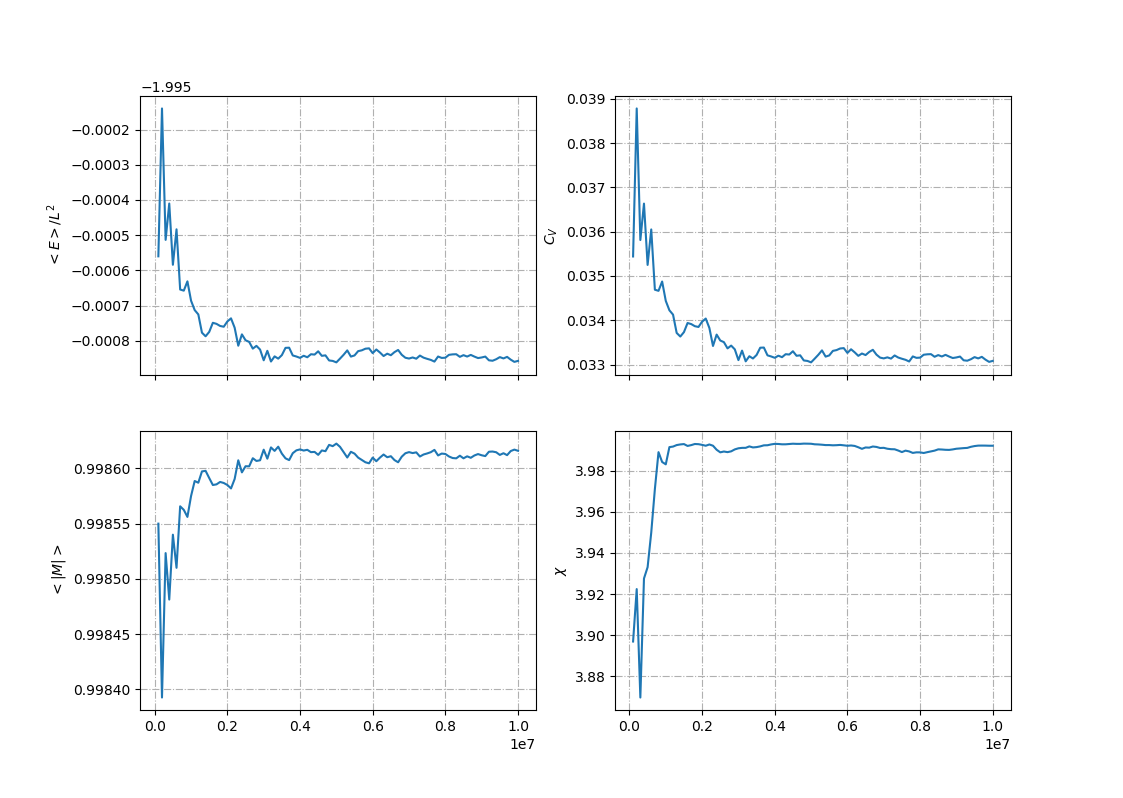
\includegraphics[scale=.5]{../Results/initial_tests.png} 
        \caption{Initial test results with $L=2$, over $10^7$ cycles, with $10^4$ cycles per data point}
        \label{fig:initial_tests}   
\end{figure}  

\subsection{Equilibrium time}
\label{SS.R.EQtime }
\subsubsection*{Augmentation of initial tests}
Figure \ref{fig:L20CV} shows $C_V$ over $7 \cdot 10^6$ cycles - which upon  inspection has a clear stable trend after $3 \cdot 10^6$ cycles  - more under discussion of results. (does not know anaylitcal). \newline

\begin{figure}[!htb]
        \centering 
         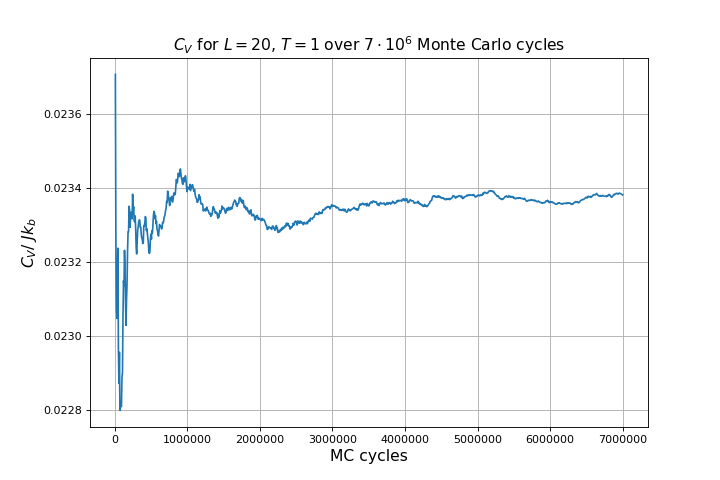
\includegraphics[scale=.55]{../Results/L20T1_CV.png} 
        \caption{Augmentation to initial test: $C_V$ using $L=20$. $10^4$ cycles per data point}
        \label{fig:L20CV}   
\end{figure} 

\subsubsection*{Initial configuration}
Figure \ref{fig:L20T1E} shows the time evolution of $\langle E \rangle$ for both a random and an ordered initial spin configuration for $T=1$. The first cycles have been omitted from the figure, as the random spin configuration starts with a very large deviation from it's equilibrium value (undesirable graph scaling). In the case of the ordered spin configuration, the expectation value fluctuates in the vicinity of $-1.99715$ for the entire duration of the simulation, with strong fluctuations before $1 \cdot 10^6$ cycles. The random configuration however produces an expectation value with a (decreasing) downwards sinking trend throughout the simulation - and with a clear offset to the ordered spin mean after $3 \cdot 10^6$ cycles. Similarly, $\langle E \rangle$ for $T=2.3$ is presented in  \ref{fig:L20T23E} - which a somewhat larger initial deviation on $\langle E \rangle$ for the ordered initial configuration than the random initial configuration, with convergence to equilibrium values offset by $\approx 0.003$ J.   \newline

In figure \ref{fig:SPIN.E.convergence} initial spin configuration on equilibrium time is examined by comparing the convergence of $\langle E \rangle$ to $\langle E \rangle_{eq}$ for each initial configuration using temperatures $T=1$ and $T=2.3$, $L=20$.  $\langle E \rangle_{eq}$ is calculated by taking the average mean of the $\langle E \rangle$ from cycle number $3\cdot 10^6$ to $4\cdot 10^6$.  As in figure \ref{fig:L20T1E} , the first cycles have been omitted. $T=1$ has a faster convergence than $T=2.3$, with the ordered configuration of $T=1$ being faster than the random configuration. For $T=2.3$, the two configurations appear to have approximately the same convergence rate, with higher fluctuations after equilibrium time than in the $T=1$ case. The configurations' effects on $\langle |M| \rangle$ follows the same trends, as is evident by figure \ref{fig:SPIN.M.convergence}. \newline



\begin{figure}[!htb]
        \centering 
         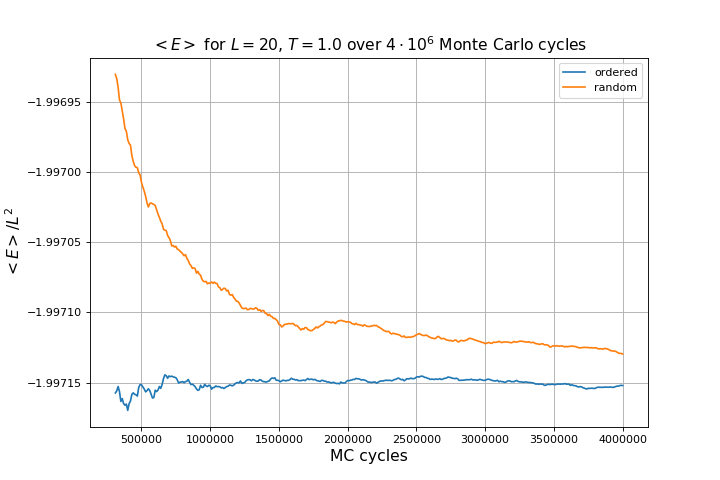
\includegraphics[scale=.55]{../Results/L20T1_eq_E.png} 
        \caption{$\langle E \rangle$ for $T=1$ - ordered vs random initial configuration}
        \label{fig:L20T1E}   
\end{figure} 

\begin{figure}[!htb]
        \centering 
         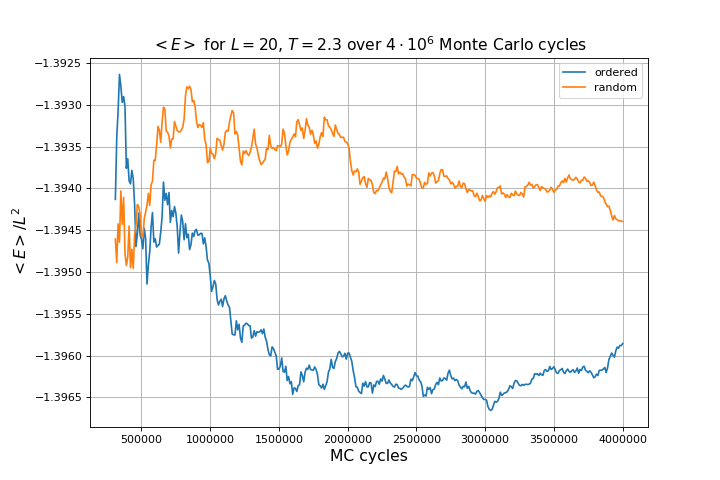
\includegraphics[scale=.55]{../Results/L20T23_E.png} 
        \caption{$\langle E \rangle$ for $T=2.3$ - ordered vs random initial configuration}
        \label{fig:L20T23E}   
\end{figure} 

\begin{figure}[!htb]
        \centering 
         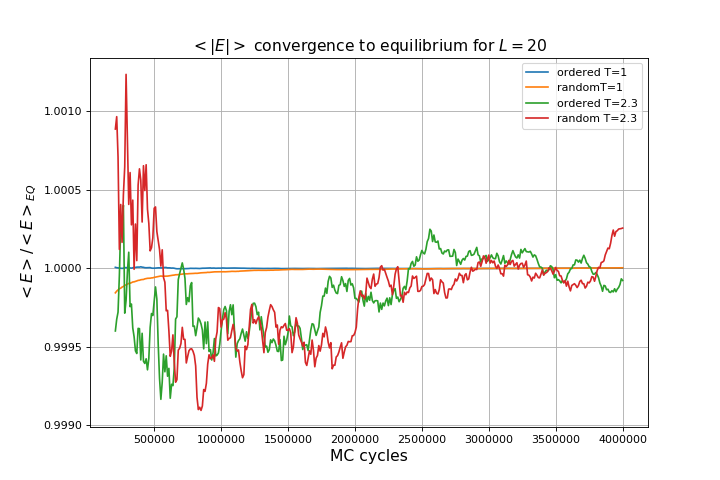
\includegraphics[scale=.55]{../Results/Econvergence.png} 
        \caption{Comparison of convergence to $<|E|>_{eq}$ for ordered and random initial configuration, with $T=1$ and $T=2.3$}
        \label{fig:SPIN.E.convergence}   
\end{figure} 

\begin{figure}[!htb]
        \centering 
         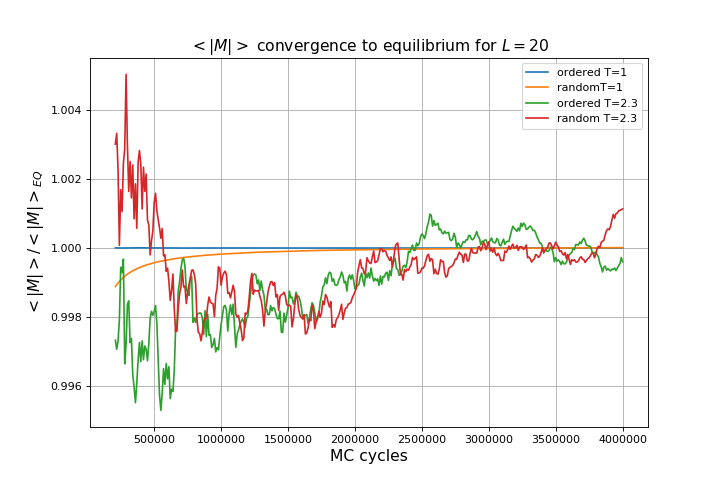
\includegraphics[scale=.55]{../Results/Mconvergence.png} 
        \caption{Comparison of convergence to $<|M|>_{eq}$ for ordered and random initial configuration, with $T=1$ and $T=2.3$}
        \label{fig:SPIN.M.convergence}   
\end{figure} 


Figures \ref{fig:SPIN.configsT1} and \ref{fig:SPIN.configsT23}, show the average number of accepted spins per lattice sweep as a function of the number of cycles is presented for $T=1$, $T=2.3$ and both initial spin configurations. For $T=1$, the number of accepted configurations per sweep is significantly higher for the random spin configuration than for the ordered configuration - especially at the start of the simulation (first values are again omitted due to scaling). Both configurations stabilize after $\approx 2 \cdot 10^6$ cycles. In the case of $T=2.3$, the number of accepted spins per sweep is approximately the same for both configurations, and two orders of magnitudes larger than in the $T=1$ case. This fits the trend that may been seen in figure \ref{fig:SPIN.configs.temp}, which shows a clear exponential increase in average cycles per sweep after equilibrium time as a function of temperature.

\begin{figure}[!htb]
        \centering 
         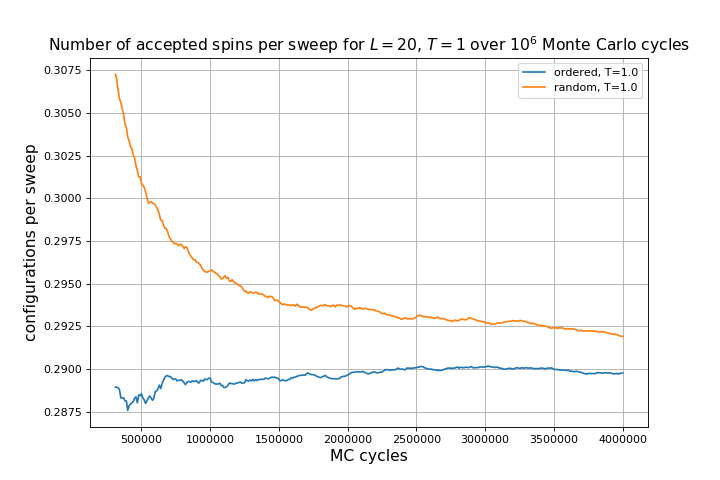
\includegraphics[scale=.55]{../Results/L20T1_acceptedconfigs.png} 
        \caption{Average (over $10^4$ cycles) number of accepted configurations per sweep for $T=1$, $L=20$, using both initial configurations}
        \label{fig:SPIN.configsT1}   
\end{figure} 
\begin{figure}[!htb]
        \centering 
         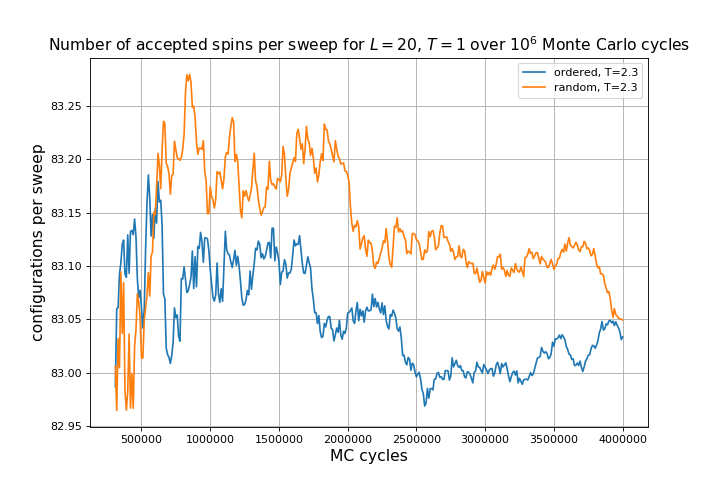
\includegraphics[scale=.55]{../Results/L20T2_acceptedconfigs.png} 
        \caption{Average (over $10^4$ cycles) number of accepted configurations per sweep for $T=1$, $L=20$, using both initial configurations}
        \label{fig:SPIN.configsT23}   
\end{figure} 


\begin{figure}[!htb]
        \centering 
         \includegraphics[scale=.55]{../Results/configs_temperature.png} 
        \caption{Average number of accepted configurations per sweep for $T=[1,2.4]$ after eq. time with a resolution of $0.3 k_B T$, $L=20$, $1 \cdot 10^6$ cycles after eq. time ($3 \cdot 10^6$) per data point.}
        \label{fig:SPIN.configs.temp}   
\end{figure} 

\subsection{Variance in energy}
\label{SS:results.VAR }
In figure \ref{fig:VAR.normalized}, the probability of each total energy level for the $L=40$ lattice with $T=1$ and $T=2.3$ is presented, based on $5000$ energy samplings in equilibrium state. It is evident that  $T=2.3$ features a much wider range of temperatures than $T=1$. For $T=1$, the energies are mainly spread out in the range $\sim [-3200,-3180] J$, with more than half of the data points around $-3200 J$, which is $\approx -2J$ per spin. In the case of $T=2.3$ the data points are roughly spread out over the range $\sim [-2300,-1900]J$, in a bell shape around $\approx -2210J$, corresponding to $\approx -1.38J$ per spin. The standard deviations, $\sigma_E$ (scaled for total energy, instead of per spin) based on the variances, $\sigma_E^2$, calculated over the equilibrium states by the program over $3 \cdot 10^5$ equilibrium cycles, are $5.47$ J and $130.6$ J, respectively for $T=1$ and $T=2.3$. \newline

The bell shape observed for $T=2.3$ roughly corresponds to the general shape expected of a Gaussian distribution. A fit to Gaussian distribution is shown in figure \ref{fig:VAR.fit}, based on $\sigma_E=131.347$ J and the mean energy, $\bar{E}=-2158.34$ J (calculated on the energy samplings). \newline

Lastly, in order to compare the observations above with $\langle E \rangle$ for $T=2.3$, a simulation using $L=20$, $T=2.3$ and 

\begin{figure}[!htb]
        \centering 
         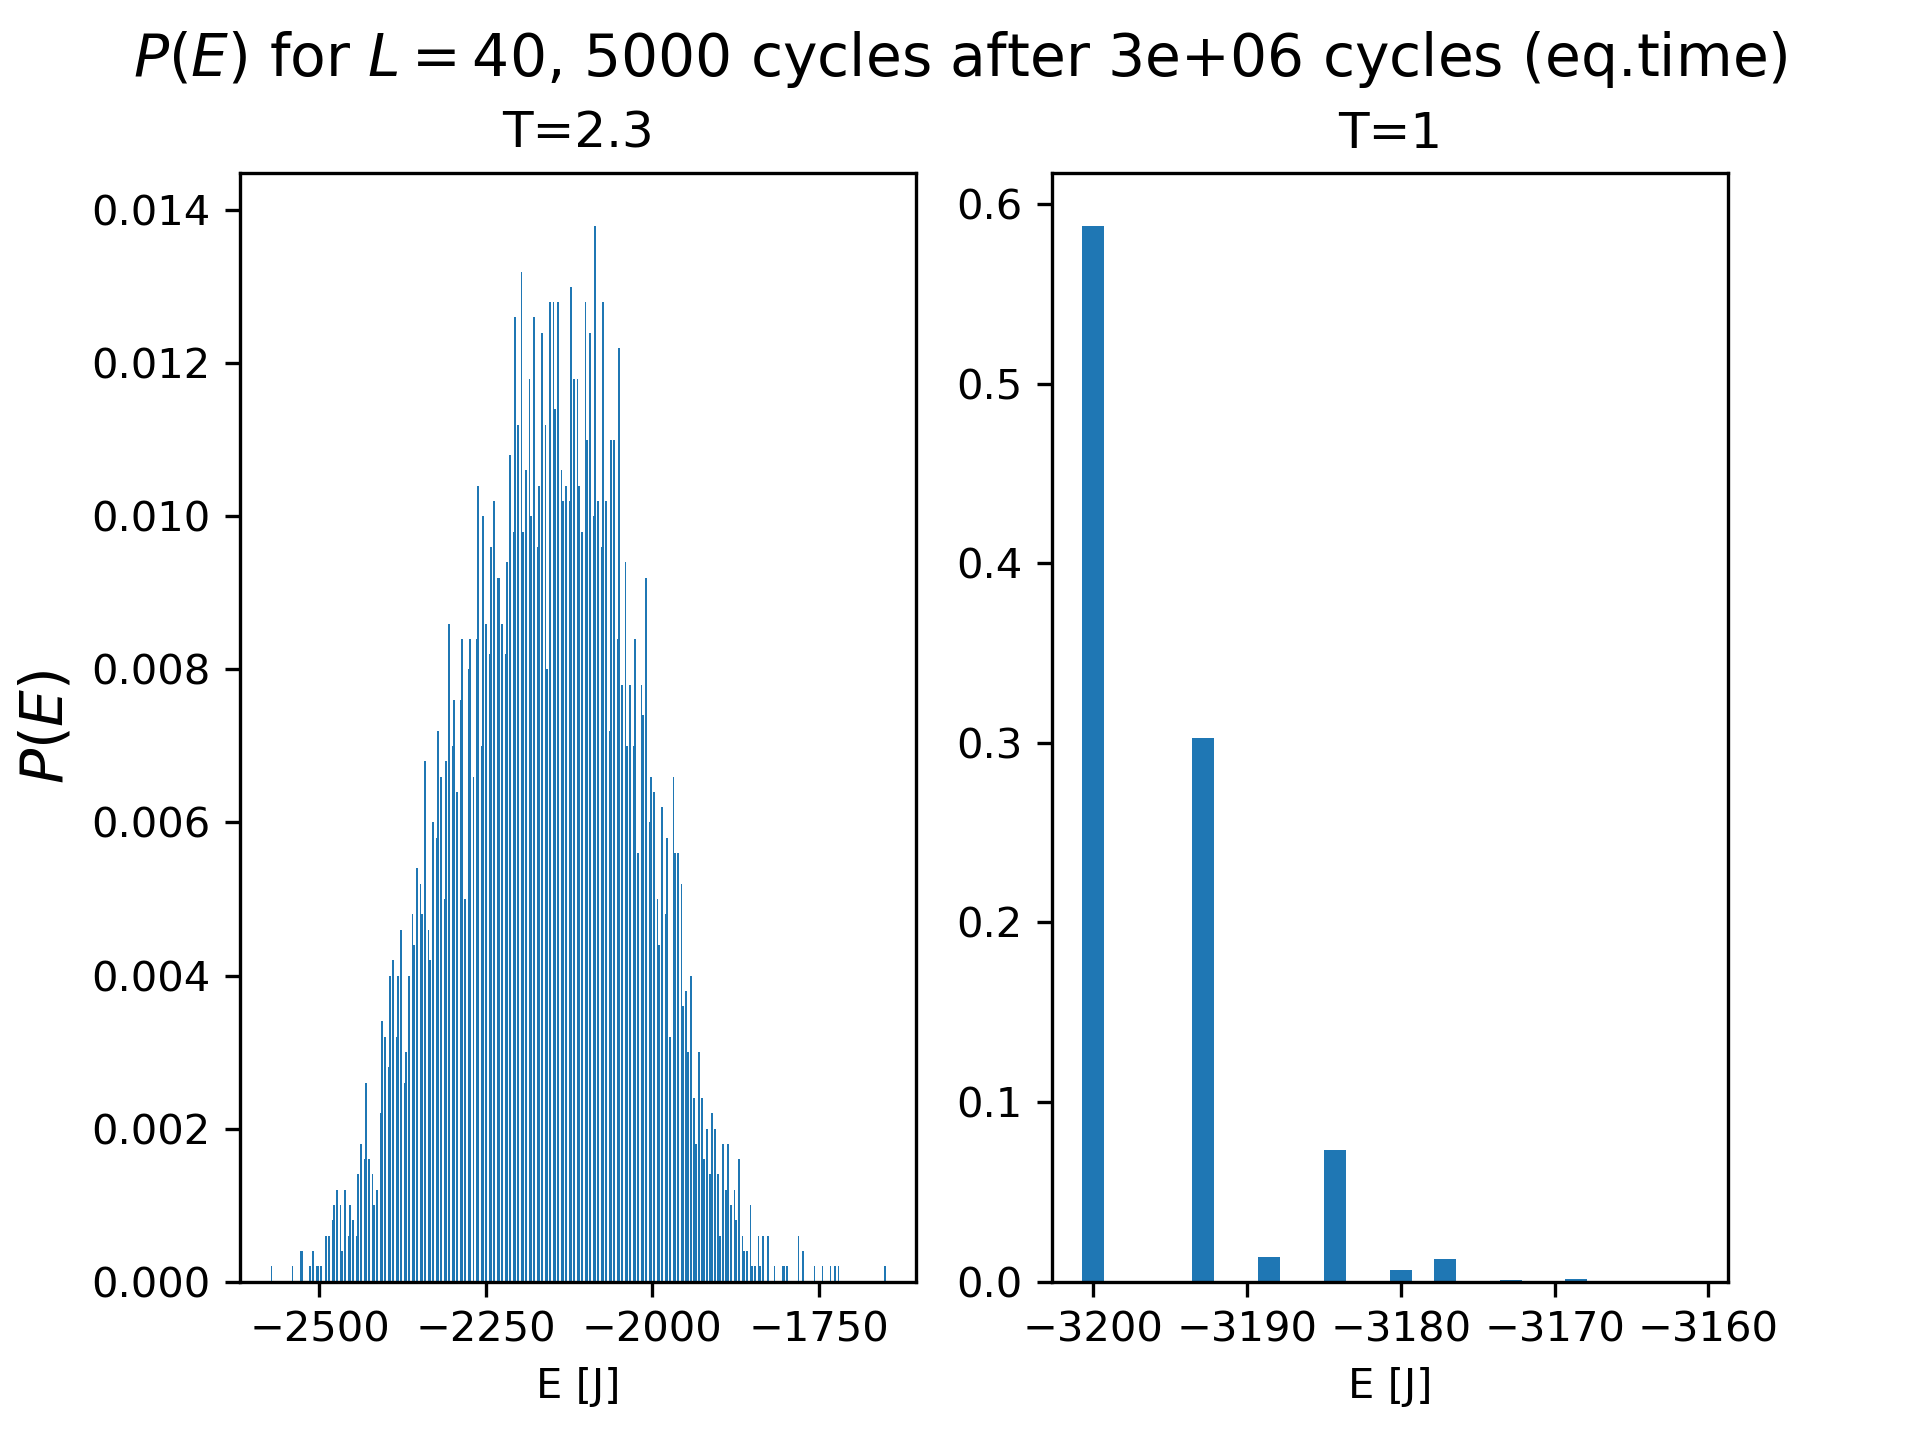
\includegraphics[scale=.7]{../Results/P(E).png} 
        \caption{Probability distribution, $P(E)$ for $T=2.3$ and $T=1$ on a $40 \times 40$ lattice, based on samplings from $5 \cdot 10^3$ cycles after equilibrium time}
        \label{fig:VAR.normalized}   
\end{figure} 


\begin{figure}[!htb]
        \centering 
         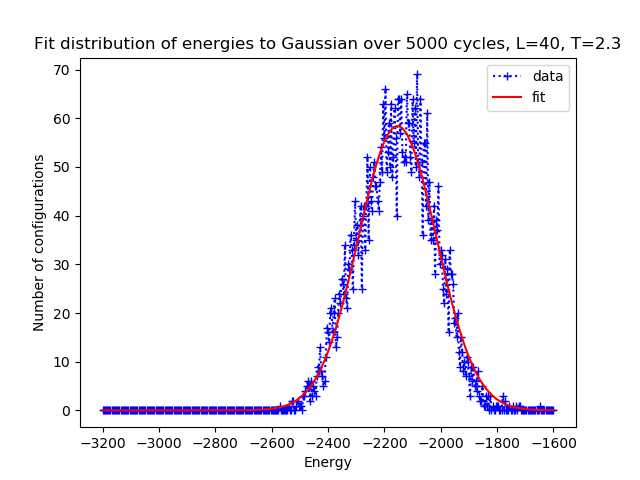
\includegraphics[scale=.7]{../Results/e_var_fit.png} 
        \caption{Probability distribution, $P(E)$ for $T=2.3$ and $T=1$ on a $40 \times 40$ lattice, based on samplings from $5 \cdot 10^3$ cycles after equilibrium time}
        \label{fig:VAR.fit}   
\end{figure}


\subsection{Estimating the Curie temperature}
\label{SS.estCurie}
\begin{figure}[!htb]
        \centering 
         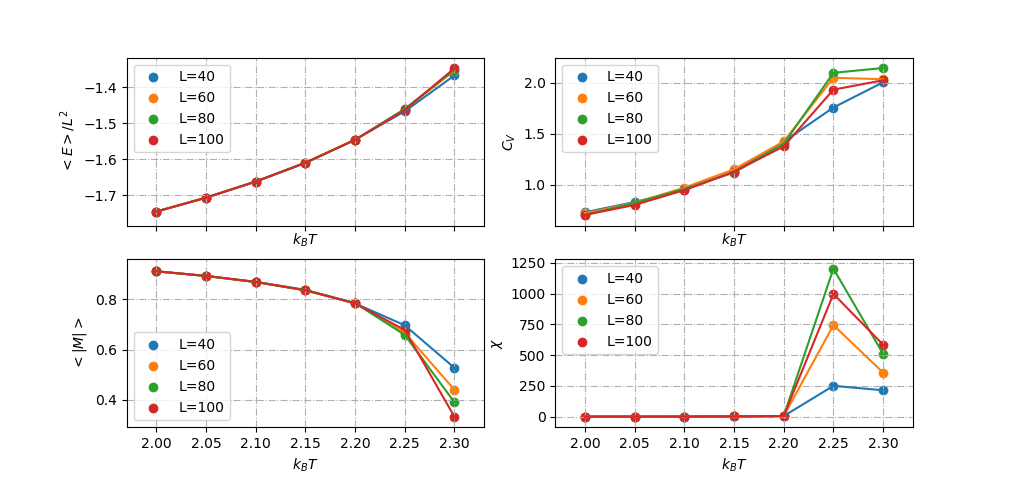
\includegraphics[scale=.6]{../Results/initial_phase.png} 
        \caption{$\langle E \rangle, C_V, \langle | M | \rangle, \chi$ as functions of $T$, with $\Delta=0.05$, for $L=40,60,80,100$ using $3.3\cdot 10^6$ cycles per temperature, with $t_{eq}=3 \cdot 10^6$.}
        \label{fig:initial_phase}   
\end{figure}

Figure \ref{fig:initial_phase} shows a clear tendency for $\langle |M| \rangle$ to decrease towards as $T$ increases, and appears to decrease faster for higher values of $L$ around $T=2.25$. Furthermore, $\chi$ increases drastically after $T=2.20$, and again especially so for higher values of $L$, where $L=80$ has the highest peak at $\chi \approx 1200$. More on this under discussion of results. As has been observed previously, $\langle E \rangle$ increases with temperature, as does $C_V$, which for higher values of $L$ increases more after $T\approx 2.2$. See \hyperref[SS.disc.var]{discussion of energy variance} for more on this.

\section{Discussion of results}
\subsection{Initial evaluation of Metropolis implementation}
\label{SS:Disucssion_init_eval}
The initial tests of the algorithm implementation indicates that the program simulates the $2x2$ lattice successfully. All parameters except $C_V$ are within a relative tolerance of $10^{-3}$ from the analytical values after $3 \cdot 10^6$ cycles. The mean of $C_V$ however is relatively inaccurate compared with the other values - whether this is due to some discrepancy in algorithm development, a consequence of the choice of mathematical model, or a statistical phenomenon is unclear . \newline

After approximately $6 \cdot 10^6$ cycles, $C_V$ appears to stabilize - albeit around a value $0.001$ higher than the analytical value. It is not unlikely that such an offset is a consequence of summing up from the beginning of the simulation - which may lead to an accumulation of unrepresentative values during the first cycles - and may very well have affected all parameters to one degree on another. Increasing the total number of cycles will result in a gradual decrease of this offset. Another solution is to not record any mean values prior to the equilibrium time. In addition, a higher $L$ is expected to increase stability of all expectation values after equilibrium time. Thus, despite the larger relative error in $C_V$ for this number of cycles, the equilibrium time is initially estimated to $\sim 3 \cdot 10^6$ cycles, based on  figures \ref{fig:init_test_E} to \ref{fig:init_test_Cv}, and table \ref{tab:abserrors} - pending further testing of the time evolution of the system.

\subsection{Initial evaluation of Metropolis implementation}
Both $\langle E \rangle>$ and $\langle |M| \rangle$ apparently drifts further from the analytical values. This may be to some discrepancy in algorithm implementation, or it possible due to the lattice size or some other simulation paramter - further testing is needed to ascertain this for sure. As both $C_V$ and $\langle E \rangle$ direclty follows the energy of the lattice, these parameters covariate, as figure \ref{fig:init_test_E} and \ref{fig:init_test_Cv} show. The initial offset that is gradually decreased is likely the results of the inclusion of energy values prior to the equilibrium state in calculating the expectation values. More on this later.

\subsection{Equilibrium time}
\label{SS:Disucssion_eqtime}
$C_V$ had a relative error $10$ times larger than $\chi$ during the initial tests, and significantly stronger fluctuations after the estimated equilibrium time of $3 \cdot 10^6$.  Comparison with analytical values for an $L=20$ lattice is however not possible, or at least feasible, so evaluation relies on stability of mean and magnitude of fluctuations alone. This is also why the augmentation test was carried out using $T=1$, as this temperature should have a relatively low variance. Upon examining $C_V$'s fluctuations for an $L=20$ lattice, it appears that the initial equilibrium time estimation is sufficient with regards to variance for equilibrium cycles.  Thus, $3 \cdot 10^6$ cycles is kept as the estimate for the number of cycles needed to obtain an equilibrium state. \newline

For the comparison of initial spin configurations on equilibrium time, it is clear that in the case of $T=1$ random initial configuration requires a significantly higher number of cycles to reach expectation values in the vicinity of those pertaining to an equilibrium state. On the other hand, this is not the case for $T=2.3$ - where both configuration have approximately the same number of sweeps per cycle and convergence rate to $\langle E \rangle_{eq}$ and $\langle M \rangle_{eq}$. For $T=1$, the two configurations are offset after $3\cdot 10^6$ cycles, which is likely to be the result of the relatively high start values of the random configuration. This may however be overcome by discarding values generated prior to the equilibrium state. As $T=2.3$ is the highest temperature used in this project, the ordered initial spin configuration is maintained as the standard initialized configuration in this project. Lastly, the mean number configurations per sweep (after equilibrium time) increases exponentially with $T$, as is to be expected - a natural consequence of the sampling rule mentioned under \hyperref[SS:M.Eq.time]{Equilibrium time in the Methods section}.

\subsection{Variance in energy}
\label{SS.disc.var}
Based on the observations in \hyperref[SS:results.VAR]{Variance in energy} under the Results section, it is evident that the energy is generally much higher for the $T=2.3$ case. This fits well with earlier observed difference in $\langle E \rangle$ for the two temperatures based on figures \ref{fig:L20T1E} and \ref{fig:L20T23E} for the $L=20$ lattice. The approximate ranges of values, $[-3200,-3180]$ and $[-2300,-1900]$ for $T=1$ and $T=2.3$, corresponds well to the simulation returns for $\sigma_E$ - $5.47$ J and $130.6$ J, considering that $2\sigma$ should cover about $.68$ of the data points.  \newline

$T=2.3$ has, as previously mentioned, a significantly larger variance in energy than $T=1$. This is directly related to the already observed tendency for higher higher energies to accept a larger number of configurations, which means that a wider range of energies is stochastically feasible as the temperature increases. Lastly, the Gaussian distribution fit may indicate that the energy of the ferromagnet, using the Ising model, goes towards a Gaussian distribution for high temperatures. More testing is however needed in order establish this with any certainty.


\subsection{Estimating the Curie temperature}
As described under the presentation of results, $\langle |M| \rangle$ decreases , and $\chi$ increases, distinctively after $T=2.25$.  The fact that higher values of $L$ exhibit this behaviour more strongly may indicate phase transitions in the range $T=[2.2,2.3]$. $\chi$ spikes at approximately $T=2.25$ for all values of $L$. However, this does not necessarily mean that $T_C\approx T=2.25$, due to the temperature resolution of the graph ($\Delta T=0.05$).



\section{Conclusions}
$3 \cdot 10^6$ cycles, $\langle E \rangle \approx -1.9960 \pm 0.0001$, $C_V \approx 0.032 \pm 0.0001$, $\chi \approx 3.99 \pm 0.005$, while $\langle |M| \rangle \approx 0.99865 \pm 0.00005$. More on this under discussion of results. 

\bibliographystyle{plain}
\bibliography{ref}


\end{document}





% ------------------- end of main content ---------------



